\documentclass[a4paper, 12pt]{extarticle}
\usepackage{fontspec}
\usepackage{polyglossia}
\setmainfont{CMU Serif}
\newfontfamily{\cyrillicfont}{CMU Serif}
\setsansfont{CMU Sans Serif}
\newfontfamily{\cyrillicfontsf}{CMU Sans Serif}
\setmonofont{CMU Typewriter Text}
\newfontfamily{\cyrillicfonttt}{CMU Typewriter Text}
\setdefaultlanguage{russian}
\usepackage[left=1cm,right=1cm,
top=2cm,bottom=2cm]{geometry}
%%% Дополнительная работа с математикой
\usepackage{amsfonts,amssymb,amsthm,mathtools} % AMS
\usepackage{amsmath}
\usepackage{icomma} % "Умная" запятая: $0,2$ --- число, $0, 2$ --- перечисление

%% Шрифты
\usepackage{euscript} % Шрифт Евклид
\usepackage{mathrsfs} % Красивый матшрифт

%% Свои команды
\DeclareMathOperator{\sgn}{\mathop{sgn}}


%% Перенос знаков в формулах (по Львовскому)
\newcommand*{\hm}[1]{#1\nobreak\discretionary{}
	{\hbox{$\mathsurround=0pt #1$}}{}}

%%% Работа с картинками
\usepackage{graphicx}  % Для вставки рисунков
\graphicspath{{Изображения/}{image}}  % папки с картинками
\setlength\fboxsep{3pt} % Отступ рамки \fbox{} от рисунка
\setlength\fboxrule{1pt} % Толщина линий рамки \fbox{}
\usepackage{wrapfig} % Обтекание рисунков и таблиц текстом

%%% Работа с таблицами
\usepackage{array,tabularx,tabulary,booktabs} % Дополнительная работа с таблицами
\usepackage{longtable}  % Длинные таблицы
\usepackage{multirow} % Слияние строк в таблице
\usepackage{lscape}
\usepackage{enumitem, kantlipsum}
\setlength{\columnsep}{1cm}
\usepackage[left=1cm,right=1cm, top=0.5cm, bottom=0.5cm]{geometry}
\pagestyle{empty} % нумерация выкл.
\begin{document}
\begin{landscape}
    \begin{multicols}{3}
        \textbf{Тест 1. «Нарисуйте картинку».}
        Дорисуйте к картинке всё, что вы считаете нужным. 
        
        \begin{center}
            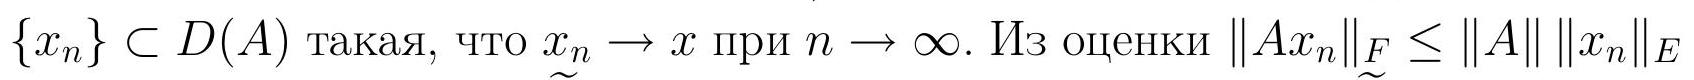
\includegraphics[scale=0.3,angle=90]{1.pdf}
        \end{center}

        \textbf{Тест 2. «Завершение фигуры».} 
        Дорисуйте десять 
        незаконченных фигур. А так же 
        придумать название к каждому рисунку. 
        \columnbreak

        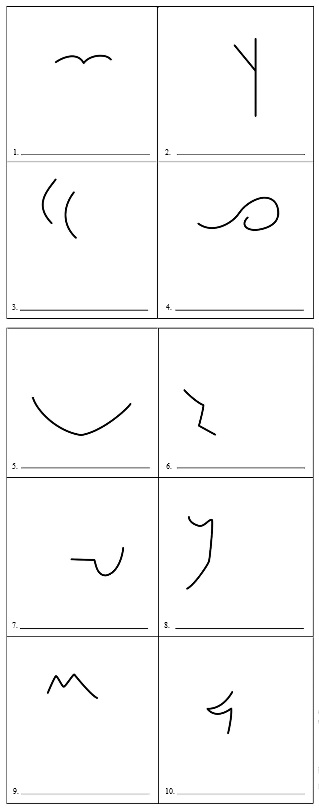
\includegraphics[width=0.4\textwidth]{test-torrens.jpg}
        
        \textbf{Тест 3. «Повторяющиеся линии».}
       
        Поверните лист на 90 градусов и основе каждой пары линий создайте
        какой-либо \textbf{не повторяющийся} рисунок.

        \includegraphics[width=0.4\textwidth, height=15.5cm]{test-torrens-4.pdf}
        
        После прохождения тестов передайте лист вашему соседу для проверки.
        \newpage
        
    \scriptsize{ «Беглость» - характеризует творческую продуктивность человека. 
    Оценивается только во 2 и 3 Тестах в соответствии со следующими правилами:
\begin{enumerate}[noitemsep,topsep=0pt,parsep=0pt,partopsep=-20pt]
    \item  При подсчете показателя учитываются только адекватные ответы.
    Если рисунок из-за своей неадекватности не получает балл по «беглости», то 
    он исключается из всех дальнейших подсчетов. Неадекватными признаются 
    следующие рисунки:
    рисунки, при создание которых предложенный стимул (незаконченный рисунок 
    или пара линий) не был использован как составная часть изображения.
    рисунки, представляющие собой бессмысленные абстракции, имеющие 
    бессмысленное название.
    осмысленные, но повторяющиеся несколько раз рисунки считаются за один ответ.
    \item   Если две (или более) незаконченных фигур в Тесте 2 использованы 
    при создании одной картинки, то начисляется количество баллов соответствующее 
    числу используемых фигур, так как это необычный ответ.
    \item  Если две (или более) пары параллельных линий в Тесте 3 использованы 
    при создании одной картинки, то начисляется только один балл, так как 
    выражена одна идея.  
\end{enumerate}


«Оригинальность» - самый значимый показатель креативности.Подсчитывается по всем трём Тестам в соответствии с правилами:
\begin{enumerate}[noitemsep,topsep=0pt,parsep=0pt,partopsep=0pt]
    \item  Оценка за «оригинальность» основывается на статистической редкости ответа. Обычные, часто встречающиеся ответы оцениваются в 0 баллов, все остальные в 1 балл.
    \item  Оценивается рисунок, а не название!
    \item  Общая оценка за оригинальность получается в результате сложения оценок по всем рисункам.
\end{enumerate}

\begin{enumerate}[noitemsep,topsep=0pt,parsep=0pt,partopsep=0pt]
    \item — цифра(-ы), буква(-ы), очки, лицо человека, птица (любая), яблоко.
    \item — буква(-ы), дерево или его детали, лицо или фигура человека, метелка, рогатка, цветок, цифра(-ы).
    \item — цифра(-ы), буква(-ы), звуковые волны (радиоволны), колесо (колеса), месяц (луна), лицо человека, парусный корабль, лодка, фрукт, ягоды.
    \item — буква(-ы), волны, змея, знак вопроса, лицо или фигура человека, птица, улитка (червяк, гусеница), хвост животного, хобот слона, цифра(-ы).
    \item — цифра(-ы), буква(-ы), губы, зонт, корабль, лодка, лицо человека, мяч (шар), посуда.
    \item — ваза, молния, гроза, ступень, лестница, буква(-ы), цифра(-ы).
    \item — цифра(-ы), буква(-ы), машина, ключ, молот, очки, серп, совок (ковш).
    \item — цифра(-ы), буква(-ы), девочка, женщина, лицо или фигура человека, платье, ракета, цветок.
    \item — цифра(-ы), буква(-ы), волны, горы, холмы, губы, уши животных.
    \item  — цифра(-ы), буква(-ы), елка, дерево, сучья, клюв птицы, лиса, лицо человека, мордочка животного.
\end{enumerate}

Тест 3: книга, тетрадь, бытовая техника, гриб, дерево, дверь, дом, забор, карандаш, коробка, лицо или фигура человека, окно, мебель, посуда, ракета, цифры.

«Абстрактность названия» — выражает способность выделять главное, 
способность понимать суть проблемы, что связано с мыслительными 
процессами синтеза и обобщения. Этот показатель подсчитывается в 
Тестах 1 и 2. Оценка происходит по шкале от 0 до 3.
0 баллов: Очевидные названия, простые заголовки (наименования), 
констатирующие класс, к которому принадлежит нарисованный объект. 
Эти названия состоят из одного слова, например: «Сад», «Горы», 
«Булочка» и т.п.
1 балл: Простые описательные названия, описывающие конкретные свойства 
нарисованных объектов, которые выражают лишь то, что мы видим на рисунке, 
либо описывают то, что человек, животное или предмет делают на рисунке, 
или из которых легко выводятся наименования класса, к которому относится 
объект — «Мурка» (кошка), «Летящая чайка», «Новогодняя елка», «Саяны» (горы), 
«Мальчик болеет» и т.п.
2 балла: Образные описательные названия «Загадочная русалка», 
«SOS», названия описывающие чувства, мысли «Давай поиграем»…
3 балла: абстрактные, философские названия. Эти названия выражают суть рисунка, 
его глубинный смысл «Мой отзвук», «Зачем выходить от туда, куда ты вернешься вечером».

«Сопротивление замыканию» - отображает «способность длительное время 
оставаться открытым новизне и разнообразию идей, достаточно долго 
откладывать принятие окончательного решения для того, чтобы 
совершить мыслительный скачок и создать оригинальную идею». 
Подсчитывается только в Тесте 2. Оценка от 0 до 2 баллов.
0 баллов: фигура замыкается самым быстрым и простым способом
1 балл: Решение превосходит простое замыкание фигуры. 
Если детали добавляются 
только внутри замкнутой фигуры, то ответ равен 0 баллов.
2 балла: фигура не замыкается вообще, оставаясь 
открытой частью рисунка или фигура замыкается с помощью 
сложной конфигурации. Два балла так же присваивается в случае, 
если фигура остается открытой частью закрытой фигуры. 
Буквы и цифры - соответственно 0 баллов.

«Разработанность» — отражает способность детально разрабатывать придуманные 
идеи. Оценивается во всех трех Тестах. Принципы оценки:
\begin{enumerate}[noitemsep,topsep=0pt,parsep=0pt,partopsep=0pt]
    \item  Один балл начисляется за каждую существенную деталь рисунка 
    дополняющую исходную фигуру, при этом детали, 
    относящиеся к одному и тому же классу, оцениваются только 
    один раз, например, у цветка много лепестков — все лепестки 
    считаем как одну деталь. Например: цветок имеет сердцевину 
    (1 балл), 5 лепестков (+1 балл), стебель (+1), два листочка (+1), 
    лепестки, сердцевина и листья заштрихованы (+1 балл) итого: 
    5 баллов за рисунок.
    \item  Если рисунок содержит несколько одинаковых предметов, 
    то оценивается разработанность одного из них + еще один балл 
    за идею нарисовать другие такие же предметы. Например: в саду 
    может быть несколько одинаковых деревьев, в небе — одинаковые 
    облака и т.п. По одному дополнительному баллу дается за каждую 
    существенную деталь из цветков, деревьев, птиц и один балл за идею 
    нарисовать таких же птиц, облака и т.п.
    \item . Если предметы повторяются, но каждый из них имеет 
    отличительную деталь, то необходимо дать по одному баллу за 
    каждую отличительную деталь. Например: цветов много, но у 
    каждого свой цвет — по одному новому баллу за каждый цвет.
    \item  Очень примитивные изображения с минимальной «разработанностью» 
    оцениваются в 0 баллов.
    \end{enumerate}  }\newcolumn
    \begin{center}
        \large{
        \vspace*{1.5cm}
 
        \textbf{Тест на креативность Торренса}
 
        \vspace{1cm}
        Предназначен для взрослых,\\
        школьников
        и детей \\от 5 лет
             
        \vspace{2cm}
        Брошюра составлена и сверстана\\
        \textbf{Суматохиной Александрой}

 
        \vfill
                        
        \vspace{0.5cm}

        
\includegraphics[width=0.4\textwidth]{page.jpg}
             
        \vspace{0.5cm}
        
        ФГБОУ ВО «Воронежский государственный университет»\\
        06.10.2022}
        \vspace*{2cm}
             
    \end{center}
\end{multicols} 
\end{landscape}
\end{document}